\chapter{Fonctionnalités}

Il nous est impossible de recenser et décrire toutes les fonctionnalités disponibles sous Galaxy. Nous nous limiterons donc la description des fonctionnalités aux principales ainsi qu'à l'ajout de plug-ins, permettant ainsi une personnalisation, ainsi que l'utilisation des workflows.

\section{Présentation générale}

Les outils de Galaxy peuvent être classés en quatre grande catégories.
\begin{enumerate}
\item Manipulation de fichiers :
	\begin{itemize}
	\item ouverture de fichiers volumineux,
	\item ajout/suppression de lignes,
	\item concaténation, filtrage, intersection,
	\item etc ...
	\end{itemize}
\item Opérations sur les données :
	\begin{itemize}
	\item addition, soustraction, moyenne, calcul de taille de séquences,
	\item conversion, formatage,
	\item etc ...
	\end{itemize}
\item Analyse de séquences :
	\begin{itemize}
	\item calcul de corrélation,
	\item recherche d'orthologues,
	\item utilisation des outils d'EMBOSS\footnote{European Molecular Biology Open Software Suite : suite logicielle dédiée aux analyses bioinformatiques},
	\item etc ...
	\end{itemize}
\item Visualisation des données :
	\begin{itemize}
	\item alignements multiples,
	\item distribution de données (histogramme, scatterplot),
	\item arbres phylogéniques,
	\item etc ...
	\end{itemize}
\end{enumerate}

\newpage
\section{Ajout de plug-ins}

L'ajout de plug-ins est une fonctionnalité uniquement disponible pour Galaxy installé localement. Pour implémenter une fonctionnalité, il faut commencer par développer le script/programme qui fera office de plug-in puis l'intégrer dans la liste des outils.

\subsection{Création}

Même si le cœur de Galaxy est dépendant Python, son architecture lui permet de gérer des scripts écrits dans différents langages de programmation interprétés\footnote{Tels que : Python, Ruby, Perl, Bash, etc ...} mais aussi compilés\footnote{Tels que : C, C++, Java, etc ...}. Cet avantage permet à (presque) tous les programmeurs de développer des outils dans leurs langages favoris, et de les intégrer en toute transparence dans Galaxy.\\

La communication Galaxy/fichiers est simple car fait intervenir les flux d'entrée/sortie en les redirigeant automatiquement vers :
\begin{itemize}
\item les fichiers intégrés dans Galaxy pour le flux d'entrée,
\item la fenêtre de résultats pour le flux de sortie.\\
\end{itemize}

Il n'est donc pas nécessaire de préparer une configuration spéciale puisque elle est réalisée par Galaxy.

\subsection{Intégration}

Afin de distinguer et de recenser tous les outils qui lui sont disponible, le logiciel possède une base de données de plug-ins sous la forme d'un fichier XML : \textit{tool\_conf.xml}.\\

\textit{tool\_conf.xml} agit en réalité comme une liste de pointeur : chaque plug-ins est identifié par un nom, un identifiant et un fichier XML qui correspond à un fichier de configuration. Pour faire savoir qu'un nouveau script est disponible, il suffit d'ajouter les lignes génériques :

\lstset{language=XML}
\begin{lstlisting} [morekeywords={section,tool}]
<section name="MyTools" id="mTools">
    <tool file="myTools/toolExample.xml" />
 </section>
 \end{lstlisting} 
 
Avec les attributs : 
\begin{itemize}
\item name : nom de l'outil tel qu'il apparaitra dans l'interface de Galaxy,
\item id : identifiant de l'outil,
\item file : chemin vers le fichier de configuration XML.\\
\end{itemize}

Il est conseillé, pour des raisons pratiques, de créer un répertoire contenant les scripts de l'utilisateur afin de les différencier des autres.\\ Dans l'exemple précédent, le futur plug-in ainsi que son fichier de configuration (\textit{toolExample.xml}) devront être placés dans un dossier \textit{tools/myTools} que l'utilisateur devra préalablement créer.\\

\newpage
\textit{toolExample.xml} doit au moins contenir les informations suivantes\footnote{Basé sur le tutorial : http://wiki.g2.bx.psu.edu/Admin/Tools/Add\%20Tool\%20Tutorial} : 

\lstset{language=XML}
\begin{lstlisting} [morekeywords={description,command,inputs,param,inputs,input,output,outputs,data,tests,test,help,tool}]
<tool id="fa_gc_content_1" name="Compute GC content">
  <description>for each sequence in a file</description>
  <command interpreter="perl">toolExample.pl $input $output</command>
  <inputs>
    <param format="fasta" name="input" type="data" label="Source file"/>
  </inputs>
  <outputs>
    <data format="tabular" name="output" />
  </outputs>

  <tests>
    <test>
      <param name="input" value="fa_gc_content_input.fa"/>
      <output name="out_file1" file="fa_gc_content_output.txt"/>
    </test>
  </tests>

  <help>
This tool computes GC content from a FASTA file.
  </help>
</tool>
 \end{lstlisting} 

Dans cet exemple, l'outil implémenté est un script Perl qui calcule le GC\%. Ce script prend 2 argument lors de son exécution : \$input (associé à un fichier interne au format fasta) et \$output (associé à la sortie standard de Galaxy : la fenêtre de résultats (Fig XX, XX et XX).\\




\begin{figure}[!h]
   \begin{minipage}[b]{0.40\linewidth}
      \centering 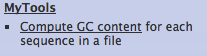
\includegraphics[scale=0.7]{Images/Ongletmytools.png}
      \caption{Onglet de l'outil implémenté.}
   \end{minipage}\hfill
   \begin{minipage}[b]{0.48\linewidth}   
      \centering 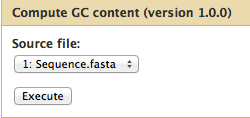
\includegraphics[scale=0.5]{Images/Gccontent.png}
      \caption{Fenêtre de l'outil implémenté.}
   \end{minipage}
\end{figure}

 \begin{figure}[!h]
 \centering
\fbox{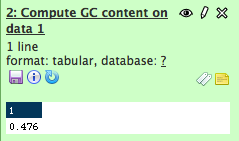
\includegraphics[scale=0.6]{Images/Resultatgc.png}}
\caption{Résultat du script \textit{toolExample.pl}.}
\end{figure}

Nous pouvons ainsi résumer les opérations nécessaires à l'intégration d'un plug-in de la façon suivante : 
\begin{enumerate}
\item écrire le script,
\item modifier \textit{tool\_conf.xml},
\item créer le fichier de configuration XML.
\end{enumerate}